
%     %%%%%%%%%%%%%%%
%
%     P A C K A G E S
%
%     %%%%%%%%%%%%%%%

\documentclass[11pt, a4paper]{article}
\usepackage{fontspec}
\usepackage{caption}
\usepackage{mathtools}
\usepackage{gensymb}
\usepackage{float}
\usepackage{comment}

% DOCUMENT LAYOUT
\usepackage{geometry}
\geometry{a4paper, textwidth=42em, textheight=70em, marginparsep=0.5em, marginparwidth=3.5em}
\setlength\parindent{0em}
\setlength\parskip{0.75em}
\captionsetup{width=0.8\textwidth}

% FONTS
\usepackage[usenames,dvipsnames]{xcolor}
\usepackage{xunicode}
\usepackage{xltxtra}
\defaultfontfeatures{Mapping=tex-text}
%\setromanfont [Ligatures={Common}, Numbers={OldStyle}, Variant=01]{Linux Libertine O}
%\setmonofont[Scale=0.8]{Monaco}
%%% modified by Karol Kozioł for ShareLaTeX use
\setmainfont[
  Ligatures={Common}, Numbers={OldStyle}, Variant=01,
  BoldFont=LinLibertine_RB.otf,
  ItalicFont=LinLibertine_RI.otf,
  BoldItalicFont=LinLibertine_RBI.otf
]{LinLibertine_R.otf}
\setmonofont[Scale=0.8]{DejaVuSansMono.ttf}

% HEADINGS
\usepackage{sectsty}
\usepackage[normalem]{ulem}
\sectionfont{\mdseries\upshape\Large}
\subsectionfont{\mdseries\scshape\normalsize}
\subsubsectionfont{\mdseries\upshape\normalsize}

\renewenvironment{abstract}{%
{\mdseries\scshape\Large\abstractname}
\vspace{1em}\\
}{\par\noindent}


\usepackage[superscript]{cite}

% LISTINGS
\usepackage{listings}
\usepackage{color}
\usepackage{appendix}

\usepackage{color}
\definecolor{codered}{rgb}{0.61,0.21,0.18}
\definecolor{codegreen}{rgb}{0,0.6,0}
\definecolor{codegray}{rgb}{0.5,0.5,0.5}
\definecolor{codepurple}{rgb}{0.58,0,0.82}
\definecolor{backcolour}{rgb}{1.0,1.0,1.0}
\lstset{
  backgroundcolor=\color{backcolour},   
  commentstyle=\color{codegray},
  keywordstyle=\color{codered},
  numberstyle=\tiny\color{codegreen},
  stringstyle=\color{codepurple},
  basicstyle=\footnotesize\ttfamily,        % the size of the fonts that are used for the code
  breaklines=true,                          % sets automatic line breaking
  keepspaces=true,                          % keeps spaces in text, useful for keeping indentation of code
  showspaces=false,                         % show spaces everywhere adding particular underscores; it overrides 'showstringspaces'
  showstringspaces=false,                   % underline spaces within strings only
  showtabs=false,                           % show tabs within strings adding particular underscores
  stepnumber=2,                             % the step between two line-numbers. If it's 1, each line will be numbered
  tabsize=4, 	                            % sets default tabsize to 2 spaces
  title=\lstname                            % show the filename of files included with \lstinputlisting
}


%     %%%%%%%%%%%%%%%
%
%     D O C U M E N T
%
%     %%%%%%%%%%%%%%%


\begin{document}
\title{IAR Task 3 Report}
\author{Angus Pearson -- s1311631\\ Jevgenij Zubovskij -- s1346981}
\date{\today}
\maketitle

%       ^v^v^v^v^v^v^v^v^v^v^v^v^v^v^v^v^v^v^v^v^v^v^v^v^v^v^v^v^v^v^v^v^v^v^v^


\begin{abstract}
 

TODO


\end{abstract}


%       ^v^v^v^v^v^v^v^v^v^v^v^v^v^v^v^v^v^v^v^v^v^v^v^v^v^v^v^v^v^v^v^v^v^v^v^

\section{Planning and Sequencing}

Using SLAM, we can now proceed to the primary goal - gathering the maximum amount of food per unit time. For that we need to be able to plan out actions, which involves calculating routes to navigate the world and sequincing them accordingly.

\subsection{Path Planning Space}
\label{Planning Space}

\textit{(Path) Planning Space} is a term used  in this document to denote the representation of the physical world in one manner or another that allows the calculation of routes routes from one pose $(X,Y, \Theta)$ to another one. This is the basis on which calculations methods are chosen \textit{\S\ref{Path Planning Algorithm}Path Planning Algorithm}. 

\subsubsection{Method Chosen}

The main mehtods\cite{path_space} of planning are seen to be used on either of the following:

\begin{itemize}
	\item \textit{Occupancy Grid}
	\item \textit{Graph (Topological Map)}
\end{itemize}


The difference between these two from the perspective of planning is the efficiency of algorithm working on the data and the pre-processing of the data going to the algorithm. Because an occupancy grid is stored on a \textit{Redis-Server} and it has very fine definition, the number of grid squares (referred to as \textit{Grid Cerlls}) is immense. Therefore, to obtain a graph representation from that, every time a path replanning would have to take place, the conversion would have to take place on a very significant number of points. Therefore, the occupancy grid was chosen due to no conversion needing to be made on the data during runtime for planning, but rather a small alteration for the \textit{Path Planning Algorithm} which should not affect the alogirithm's performance.

\subsubsection{Alterations}

The granularity of the \textit{Planning Grid (Planning Space)} did not necessarily have to match that of the occupancy grid on Redis for the following reasons:


\begin{itemize}

	\item Robot Dimensions     - the robot's dimensions are larger than the mapping (server-side) granularity
	\item Odometry Distortion  - extremely finely planned path on an occupancy grid introduces many turns, increasing odometry drift rate considerably \cite{task2_report}
	\item Runtime Optimization - as long as there is a path to the goal and the robot can follow it, we wish to save as much processing time as we humanely can and plannign with bigger cell dimensions helps us save calculation time

\end{itemize}

Hence, it as decided that the rganularity would be available for configuring as a parameter before runtime without really limiting any way because that would diminish the further possible modifications to the aglorithm. However, by defaul it is set to be equal to the granularity of the occupancy grid.

Moreover, the \textit{(Grid) Cells} store their actual $(X ,Y)$ coordinates as well as occupancy - are they free space or not. Grid cells are stored in a two dimensional array which is indexed by using actual $(X ,Y)$ coordinates. Furthermore, said array is also dynamycally expanding in both dimensions so as to accomodate any number of cells (limited only by memory capacity) in order to not miss a valid optimal path due to any array bounds which also makes this solution more extensible and easily modifiable.

Therefore, formign a local cache of the Redis server data suitable for path search computations of virtually any kind. Lastly, because the occupancy data is stored on Redis, the implementation obtains unknown occupancies from the server and caches them locally in said two-dimensional array. 


%       ^v^v^v^v^v^v^v^v^v^v^v^v^v^v^v^v^v^v^v^v^v^v^v^v^v^v^v^v^v^v^v^v^v^v^v^


\subsection{Path Planning Algorithm}
\label{Path Planning Algorihtm }

This method should allow the robot to navigate the mapped space between any two unoccupied \textit{(Grid) Cells} \textit{\S\ref{Code}} of the planning space (grid). 

\subsubsection{Research}

Firstly, there are many options for the \textit{Path Planning Algorithm} that search for a path between a goal and a destination location:

\begin{itemize}

	\item \textit{Floyd-Warshall Algorithm}\cite{path_warshall} - a many-to-many algorithm for planning routes
	\item \textit{Djikstra Algorithm}\cite{path_warshall} - a one-to-many algorithm
	\item \textit{A* Algorithm}\cite{path_astar}	- a one-to-one algorithm

\end{itemize}

These are some of the most common and robust pathing algorihtms used in pathing. However, even based on the iformation above it can be concluded that Floyd-Warshall algorithm is not waht we were lookign because w have a single strating point - the position of the robot. Moreover, empirical data\cite{path_efficiency} shows that the best-first search algorithm is considerably faster than the Djikstra algorithm and in fact is in general considered the fastest planning algorithm. Moreover, it's varioations as well as its purest form are used industry-wide in robotics. More reasons for choosing A* can be outlined in \textit{\S\ref{Path Planning Algorihtm Alterations}}

\subsubsection{Method Chosen} 

Therefore, A* was chosen to be the algorithm of choice for path calculation to the target grid cell. The pseudocode explaining its basic operation is as follows:

\begin{figure}[H]
	  \caption{The A* algorithm pseudocode\cite{path_astar_pseudocode} adapted to use the \textit{Planning Space} chosen - an occupancy grid }
 	  %\centering
	  %\lstinputlisting[language=python]{../../astar_pseudo.py}
\end{figure} 


\begin{figure}[H]
	  \caption{The A* algorithm path reconstruction pseudocode\cite{path_astar_grid_no_grid} adapted to use the \textit{Planning Space} chosen - an occupancy grid }
 	  %\centering
        %\lstinputlisting[language=python]{../../astar_path_reconstruction.py}
\end{figure} 

\subsubsection{Alterations}
\label{Path Planning Algorihtm Alterations}

The chosen \textit{\S\ref{Path Planning Algorihtm} Path Planning Algorihtm - A*} uses the movement and \textit{Heuristic Cost} to estimate the total cost of  including cell into the claculated path. Therefore, as we know the pose of each grid cell, \textit{Euclidian Distances} were chosen to be a measure of (transition) cost between cells making it the cost function betwen any two cells $A$ and $B$. The \textit{Heuristic Function (Cost)} is $10$ times the Euclidian distance from currently considered cell to the goal. The reason for such a high number is that we wish to see the algorithm converge as fast as possible while findign an adequately short path to the desired destination whcih also reduces the amount of server requests for unknown occupancies. On a side note, the movement cost is simply the sum euclidian distances between nodes along the (considered) path involvind said cell.

Secondly, the A* pseudocode had to be adapted to work on a grid instead of a graph which was solved by a simple function obtaining its neighbours by using the considered cell's pose to get its adjacent ones from the \textit{\S\ref{Path Planning Space}Occupancy Grid}.

Secondly, most iterations of the A* algorithm rely on either graphs\cite{path_astar_grid_no_grid}  or only movements up, down, left or right\cite{path_astar_grid_no_diagonals}. However, it seemed like a wasted opportunity to not allow the robot to move diagonally. Such cells are referred to as  \textit{Diagonal Cells} - cells diagonal to the currently considered cell - whose adjacent cells we wish to consider for furhter pathing for the remainded of this report and in the code comments. Moreover, it had to be also accounter for scenarios where the diagonal cell is blocked by two of its neighbours and the diagonal cell can no longer participate in path calculation as shown in the following figure.


\begin{figure}[H]
	  \caption{The \textbf{top} figure shows the $central$ cell (square) is the so called \textit{Considered Cell} whose neighbours we are trying to obtain to plan a path. The \textbf{top} figure shows that we cannot consider the \textit{Diagonal Cell} $A$ as a valid neighbour because it is blocked by $B$ and $C$ making the movement along the red arrow as seen in the \textbf{bottom} figure impossible}
 	  %\centering
    	  %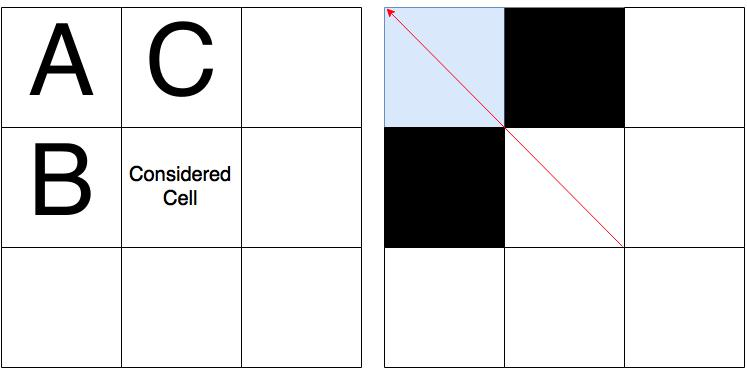
\includegraphics[width=0.5\textwidth]{fig_astar_diagonal}
\end{figure} 






%       ^v^v^v^v^v^v^v^v^v^v^v^v^v^v^v^v^v^v^v^v^v^v^v^v^v^v^v^v^v^v^v^v^v^v^v^



\subsection{The Planner}

This section is concerned with the intergation of the algorithm and data structures described above into the main control loop and its interaction with previosuly established subsystems\cite{task2_report}. The algorithm determinign the next action or travel destination and sequencing said action is called the \textit{Planner} and is, therefore, responsible for maximizing the food collection rate by sequencing events governing said rate.

\subsubsection{Method Chosen}
\label{Planner Principle}

Now that we are able to localize ourselves, knwo the map and can calculate paths on the grid, we can set priorites for action to maximize food gathering. Firstly, it is important to note that a it is considered that each \textit{Food Source} has only one unit of \textit{Food}. Upon return to the \textit{Nest} and droppign off currently collected food the robot resets the food sources which now have food units again, therefore, starting a new \textit{Food Collection Round (a.k.a. Round)}. Hence, the aciton priorites were set as follows

\begin{enumerate}
	\item \textit{Find} the first food source to begin periodic behavior in the following points
	\item \textit{Explore} once per Food Collection Round
	\item \textit{Collect} closest uncollected known / recorded food source
	\item \textit{Return} to the nest and drop off collected food
\end{enumerate}

Thus, we aim to find some food source first to start collecting food as soon as possible. After which exploration for new food sources becomes less of a priority and is only invoked once per round as we do not wish to waste too much time on exploration when we already have food to collect. Therefore, next on the list of priorities is collecting all the food before returning to the nest to drop it off because if we do not collect all the food before a new round start, it is reset - lost. After that is done, the robot returns to the nest and drops off collected food.


\begin{figure}[H]
	  \caption{The planning algorithm - the \textit{Planner} in state-diagram form, this decision making tree is implored on overy iteration of the control loop and determines the action the system is to follow}
 	  %\centering
    	  %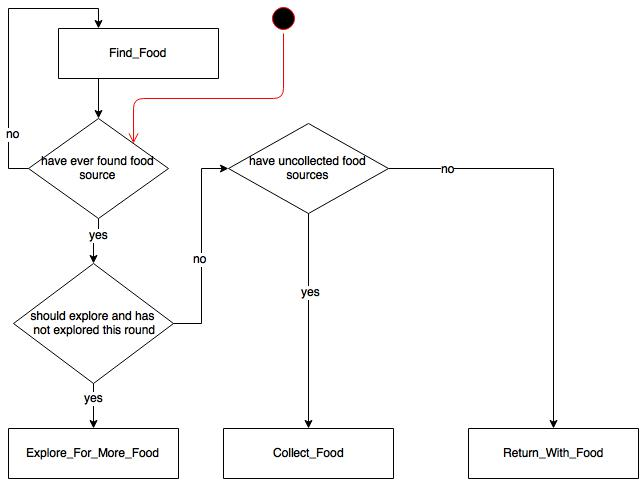
\includegraphics[width=0.5\textwidth]{fig_planner}
\end{figure} 

The robot aims to collect the closest food first (bases on Euclidian distances). The movement between cells is moevement along the vector between their recorded coordinates by adjusting the angle along the \textit{Vector of Approach}, same as \textit{Return Algorithm}\cite{task2_report}. Moreover, sometimes unxecpected events can happen that coud lead the robot away from said approach vector. Hence, the next destination is decided (as per above priority list) when the following events happen:

\begin{itemize}

	\item Food collected from a Food Source
	\item Food dropped off at nest - round finished
	\item Path lost - went a distance over the threshold away from the path

\end{itemize}

\subsubsection{Alterations}

After reviewing initial \textit{\S\ref{Experimental Results}Eperimenal Results} it was decided that due to the grid granularity being set (by default) in the same order of magnitude as robot dimensions, it is reasonable to assume that no two food sources can exist in the same grid cell as the cell sizes are assumed to be set by the user / programmer to a granularity not exceeding robot dimensions. Lastly, because the algorithm needs to find new food sources, the boredom mechanism \cite{task1_report} was reinstated into the control loop and is the exploration mechanism and is utilized during the \textit{Find} stages of the algorithm. 

%       ^v^v^v^v^v^v^v^v^v^v^v^v^v^v^v^v^v^v^v^v^v^v^v^v^v^v^v^v^v^v^v^v^v^v^v^


\subsection{User Input and Alterations}

User input for this task indicates when the robot is on top of a food source. However, this was separated into two key presses because when we first find a food source, there is no odometry or other lozalization error as we know we are physically on top of it. However, when the in the next food collection round we attempts to harvest the same food, errors accumulate, as seen in \textit{Task 2}\cite{task2_report} and therefore need to make sure we reach the food source. Therefore, another key press indicates when the robot is on top of a old food source. Such a distinction is important, because due to aforomentioned accumulation of errors, we are unsure if we are truly on top of the nest, therefore recording it as a new food source would be incorrect and updating the position of the food is not in the scope of the Planning Algorithm. 

Moreover, if the robot does not properly localize for one reason or another (such as errors discussed before) and thinks it has raeached the nest but there is no user input suggesting that is true, it beings to spiral outwards from the spot it things the food is in until user input is encountered. Therefore, ensuring that if the fodo is somewhere in the viscinity, it will be found fairly quickly again. 


TODO insert from dropbox 

\begin{figure}
	  \caption{The effects of user input on the \textit{Planner}, pressing \textit{Space} results in a new food source being 
		recorded in the current grid cell (if it was not found there before) whereas pressing \textit{Enter} tells the Plannes
		 that we are at the location of an already previously visited \textit{Food Source}}
 	  %\centering
    	  %\includegraphics[width=0.5\textwidth]{fig_planning_flow}
\end{figure} 



\subsection{Subsystem Interaction}

Lastly, the integration of the algorithm into the main system is seamless and practically mimics the integration of the \textit{Return Algorithm}\cite{task2_report} a.k.a. the \textit{Bug 2.4.1.1.2}. The difference is now we know where there is a wall and can fully relay the control to the planner, unless we are exploring using "boredom"\cite{task2_report} or are being "unstuck"\cite{task2_report} without fear of the robot crashing into the wall. 

Therefore, ensuring that SLAM and A* are the main control element in the system, unless we need to avoid collision. A further note is that the above distinction is not as clear in the \textit{\S\ref{Code} Code} because of the location of methods, however, the end result (and aim) is best summarize by the related diagram \ref{fig_planning_internal}.

Unfortunately, a picture does not introduce much mroe than saying : unless about to collide with an obstacle, the Planner determines further actions because due to mapping, unlike with the \textit{Return Algorithm}\cite{task2_report} we no longer need to stick to walls as we have mapping and know (or will know) where such are and can plan with them in mind.




%       ^v^v^v^v^v^v^v^v^v^v^v^v^v^v^v^v^v^v^v^v^v^v^v^v^v^v^v^v^v^v^v^v^v^v^v^





TODO make sure angus has a pic of waht an occupancy grid is
TODO comment somehow on the rganularity effect on performance (and do tests)
TODO make sure occupancy grid is already described in a previous section
TODO reference pictures
TODO set granularity to robot dimension
TODO insert stuff from google drive





\newpage
\begin{thebibliography}{}

\bibitem{task1_report} 
\par{IAR 2016 Task1 Report} \\
\textit{Angus Pearson, Jevgenij Zubovskij}

\bibitem{task2_report} 
\par{IAR 2016 Task1 Report} \\
\textit{Angus Pearson, Jevgenij Zubovskij}



\bibitem{path_space}
\par{Map Representation Comparison and Planning (online article)}-
\textit{http://correll.cs.colorado.edu/?p=965}



\bibitem{path_warshall} 
\par{Theory of Algorithms (lecture)}
\textit{http://cs.winona.edu/lin/cs440/ch08-2.pdf}

\bibitem{path_djikstra} 
\par{Greedy Algorithms (online article)}
\textit{http://www.geeksforgeeks.org/greedy-algorithms-set-6-dijkstras-shortest-path-algorithm/}

\bibitem{path_astar}
\par{A* Comparison (online article)}
\textit{http://theory.stanford.edu/~amitp/GameProgramming/AStarComparison.html}

\bibitem{path_efficiency} 
\par{Comparative Study of Path Planning Algorithms}
\textit{http://research.ijcaonline.org/volume39/number5/pxc3877058.pdf}

\bibitem{path_astar_pseudocode} 
\par{A* Search Algorithm (online article)}
\textit{http://web.mit.edu/eranki/www/tutorials/search/}



\bibitem{path_astar_grid_no_diagonals} 
\par{Introduction to A* (online article)}
\textit{http://theory.stanford.edu/~amitp/GameProgramming/AStarComparison.html}



\bibitem{path_astar_grid_no_grid} 
\par{A* Search Alogorith (online article)}
\textit{https://en.wikipedia.org/wiki/A*\_search\_algorithm}




\end{thebibliography}

\begin{comment}

\newpage
\begin{appendices}
\section*{Appendix}
\subsection{Code Listings}
\label{Code}
\lstinputlisting[language=python]{../../main.py}
\lstinputlisting[language=python]{../../data.py}
\lstinputlisting[language=python]{../../comms.py}
\lstinputlisting[language=python]{../../state.py}
\lstinputlisting[language=python]{../../pathing_state.py}
\lstinputlisting[language=python]{../../pathing_algorithm.py}
\lstinputlisting[language=python]{../../astar.py}
\lstinputlisting[language=python]{../../navigation_state.py}
\lstinputlisting[language=python]{../../navigation_algorithm.py}
\lstinputlisting[language=python]{../../odometry_algorithm.py}
\lstinputlisting[language=python]{../../odometry_state.py}
\lstinputlisting[language=python]{../../constants.py}
\lstinputlisting{../../requirements.txt}
\end{appendices}

\end{comment}


\end{document}
